\chapter{深度卷积神经网络}

\section{引言}
% \textcolor{red}{看之前的论文,引言先介绍基本问题,然后提出本章的解决方案,最后本章安排}

% \textcolor{red}{5518/9500。}

人工神经网络\cite{hebb2005organization}是一种通过模仿大脑神经元行为进行信息处理的数学模型,但由于其无法承受大规模的参数和训练样本并且具有泛化能力差等问题。Fukushima\cite{fukushima1982neocognitron}于1982年首次提出了卷积神经网络模型,Lecun 等人对神经网络传统算法在训练上面临的计算复杂度高等问题进行了改进,提出了基于梯度下降的优化算法\cite{lecun1998gradient}和BP算法\cite{lecun1989backpropagation}。2003年,Simard对卷积神经网络进行了简化\cite{simard2003best}。Hinton 在2006年的两篇文章\cite{hinton2006reducing,hinton2006fast}可以作为深度学习(Deep Learning,DL)正式提出的里程碑。Ciren等人\cite{ciresan2011flexible}在2011年对神经网络进行改造使其可以通过GPU进行训练计算,并在大量的图像数据集对深度学习算法进行了测试,并且都取得了最好的成绩。其在工业界以及学术界掀起了巨大的浪潮,被应用于语音识别\cite{hinton2012deep}、图像识别\cite{krizhevsky2012imagenet}和自然语音处理\cite{collobert2011natural}等各种方面。 专门针对于深度学习的芯片不断问世,例如谷歌公司的TPU\cite{jouppi2017datacenter},大大提高了深度学习的应用场景。
深度神经网络模型是一种非常强大的深度学习模型,他同时可以处理有监督和无监督学习任务。并且随着科技的发展,数据量越来越大,计算机并行能力也有了很大的提高。针对于海量数据,简单的线性模型由于无法充分利用计算能力,不再适用,可以预见在将来会有越来越多的工作应用到深度学习。目前,其内涵已经超出了传统的多层神经网络,甚至机器学习的范畴,逐渐朝着人工智能的方向快速发展\cite{silver2017mastering}。

1982年,Kunihiko等人\cite{fukushima1982neocognitron}首次将卷积神经网络模型的概念引入深度学习。后来许多学者在实践中对CNN的发展和理论分析作出了重大贡献。1989年,LeCun等人将基于梯度的学习方法\cite{lecun1998gradient}和BP算法\cite{lecun1989backpropagation}引入到CNN。2003年,Behnke写了一本总结CNN\cite{behnke2003hierarchical}的书。同年,Simard等人\cite{simard2003best}对卷积神经网络进行了简化。2011年,Ciren等\cite{ciresan2011flexible}进一步改进CNN并实现了GPU版本,使得CNN的训练识别速度有了巨大的提升,并使用CNN框架对多个图像数据库进行实验,并取得了最佳成果。

本章安排如下:2.2节对深度学习的基本分类进行了介绍,2.3节详细地阐述了传统人工神经网络结构的基本定义和神经元之间信息传递的过程,2.4节对本文主要利用的深度卷积神经网络的特性进行了介绍,2.5节进行本章总结。


\section{基本分类}
传统上可以把深度学习分为卷积神经网络(Convolutional Neural Networks, CNN)、递归神经网络(Recurrent Neural Networks, RNN)、长短时记忆网络(Long short-term memory, LSTM)、深度信念网络(Deep Belief NetWorks,DBN)、自编码器(AutoEncoder)、稀疏编码(Sparse Coding)、限制波尔兹曼机(Restricted Boltzmann Machine, RBM)等。

其中卷积神经网络是最流行的一种深度学习模型,通过使用卷积层极大地减少了中间层的参数数目,使学习效率更高并较少过拟合,同时卷积操作独有的局部感受野(local receptive fields)、共享权重(shared weights)和池化(pooling)三种特性也是处理序列元素分类识别的很重要的一点,权重共享策略减少了需要训练的参数,相同的权重可以让卷积核不受信号位置的影响来检测信号的特性,使得训练出来的模型泛化能力更强;池化运算可以降低网络的空间分辨率,从而消除信号的微小偏移和扭曲。

递归神经网络是一种包含循环的,允许信息持久化的神经网络模型。传统的前馈神经网络中,单独的输入完全确定了余下层的神经元的激活值。而对于递归神经网络,隐藏层和输出层的神经元的激活值不仅由当前的网络输入决定,而且包含了前面的输入的影响。长短时记忆网络是一种特殊的递归神经网络,主要用于解决递归神经网络前期模型难以训练的问题。其通过刻意设计的单元结构,在递归神经网络的基础上添加了元胞状态(cell state)用来保存长期的状态,然后通过门函数来控制此长期状态。

深度信念网络是一个概率生成模型,是由多个限制玻尔兹曼机组成,这些网络被“限制”为一个可见层和一个隐藏层,层间存在连接,但是层内的单元间不存在连接。隐藏单元被训练来捕捉在可见层表现出来的高阶数据的相关性。

通过对于以上几种最常用的深度学习方法的介绍,我们可以发现卷积神经网络是最适合处理本文这种静态类型的数据,循环或者说是不同时刻的输入对于地海杂波类型的识别并没有提高,故递归神经网络和长短时记忆网络显然不适合本问题。另一方面,深度信念网络的生成模型并不关心不同类别之间的最优分类面的位置,故其用于分类问题时,分类精度没有判别模型高。且其学习的是数据的联合分布,相比其他算法具有更高的复杂性。

\section{传统人工神经网络结构}

人工神经网络是一种模拟大脑神经系统的算法,其可以从海量的训练样本中学习到一个权重函数,用来进行模式识别、分类等。神经网络主要是利用将许多个单一神经元(也称作感知器)联结在一起,一个神经元的输出就可以是另一个神经元的输入,形成一个有向无环的网络结构。
首先介绍单一神经元的结构,如图\ref{fig:neural}所示,神经元一般具有多个输入$x=[x_1,x_2,\dots,x_n] $,这些输入可以取0和1中的任意值。神经元对于每一个输入有权重$w=[w_1,w_2,\dots,w_n] $ 和一个总的偏置$b_0$ ,其输出为:
\begin{equation}
  y = f(w\cdot x + b)
  \label{equ:neural}
\end{equation}
这里的 $f$为该神经元的激活函数,我们在后面进行描述。

\begin{figure}
  \centering
  \includestandalone[width=\textwidth]{figures/networks/neural}
  \caption{神经元}
  \label{fig:neural}
\end{figure}

上述多个神经元分层互联即可以形成神经网络。图\ref{fig:network}是一个简单的神经网络,其中圆圈表示神经网络的节点,也即神经元。
对于一个具有$n_l$层的神经网络,如将第$ l $层用 $ L_l$表示,则有最左边的一层$  L_1$为输入层,最右的一层$ L_{n_l} $为输出层。由于不能在训练样本集中观测到中间所有节点的值,故将这些层称做隐藏层。
本例中网络的层数$ n_l=3$,输入层具有4个输入单元,隐层具有5个隐藏单元,输出层只有一个输出单元。

\begin{figure}
  \centering
  \includestandalone[width=\textwidth]{figures/networks/network1}
  \caption{神经网络}
  \label{fig:network}
\end{figure}

根据输入 $x_i$求解输出$y$的主要过程为前向传播。
我们用$ w^{(l)}_{ij}$表示第 $ l $层的第 $ j$ 单元与第 $ l+1 $层的第$  i$ 单元之间的权重,$ b^{(l)}_i $是第$  l+1 $层中第$  i$ 单元的偏置项。
因此,$w^{(l)}$为第$l$层权重组成的向量,$ w^{(1)} \in \Re^{4\times 3}$ , $ w^{(2)} \in \Re^{1\times 5}$ 。
根据图\ref{fig:neural}和公式\ref{equ:neural}可以知道每个神经元节点的输出是经过激活函数的激活值,可以用$ y^{(l)}_i$ 表示第$  l $层的第 $ i$ 单元的输出值。
当$  l=1$ 时,$  y^{(1)}_i$为就是第$  i $个输入值,也即有$  y^{(1)}_i = x_i $。
当权重已知的时候,我们就可以根据公式\ref{equ:neural}求解此传播过程,进而求解最终的输出值$y$。
从$L_1$层到$L_2$层的过程为:
\begin{align}
  y_1^{(2)} &= f(w_{11}^{(1)}x_1 + w_{12}^{(1)} x_2 + w_{13}^{(1)} x_3 + w_{14}^{(1)} x_4 + b_1^{(1)})  \\
  y_2^{(2)} &= f(w_{21}^{(1)}x_1 + w_{22}^{(1)} x_2 + w_{23}^{(1)} x_3 + w_{24}^{(1)} x_4 + b_2^{(1)})  \\
  y_3^{(2)} &= f(w_{31}^{(1)}x_1 + w_{32}^{(1)} x_2 + w_{33}^{(1)} x_3 + w_{34}^{(1)} x_4 + b_3^{(1)})  \\
  y_4^{(2)} &= f(w_{41}^{(1)}x_1 + w_{42}^{(1)} x_2 + w_{43}^{(1)} x_3 + w_{44}^{(1)} x_4 + b_4^{(1)})  \\
  y_5^{(2)} &= f(w_{51}^{(1)}x_1 + w_{52}^{(1)} x_2 + w_{53}^{(1)} x_3 + w_{54}^{(1)} x_4 + b_5^{(1)})
  \label{equ:fp1}
\end{align}
根据同样的计算过程可以得到:
\begin{equation}
  y = y_1^{(3)} =  f(w_{11}^{(2)} y_1^{(2)} + w_{12}^{(2)} y_2^{(2)} + w_{13}^{(2)} y_3^{(2)} + w_{14}^{(2)} y_4^{(2)} + w_{15}^{(2)} y_5^{(2)} + b_1^{(2)})
  \label{equ:fp2}
\end{equation}
我们只需要把公式\ref{equ:fp1}代入\ref{equ:fp2}就可以计算得到输入$x_i$与输出$y$之间的关系。
为了使表达更清晰,我们用$ z^{(l)}_i $表示第$ l $层第$  i$单元输入加权和,则有:
\begin{equation}
  z_i^{(l)} = \sum_{j=1}^n w^{(l-1)}_{ij} x_j + b^{(l)}_i
\end{equation}
因此公式\ref{equ:fp1}变为
\begin{equation}
  y^{(l)}_i = f(z^{(l)}_i)
\end{equation}
则整个前向传播过程可以简化为:
\begin{align}
  z^{(l+1)} &= w^{(l)} y^{(l)} + b^{(l)}   \\
  h^{(l+1)} &= f(z^{(l+1)})
\end{align}
其中,$b^{(l)}$为第$l+1$层偏置项组成的向量,$h^{(l)}$为第$l$层各个单元输出值组成的向量。
% 这样就可以得到一种更简洁的表示法。这里激活函数 $ f(\cdot)$ 扩展为用向量(分量的形式)来表示,即$  f([z_1, z_2, z_3]) = [f(z_1), f(z_2), f(z_3)]$ ,那么,上面的等式可以更简洁地表示为:
% \begin{align}
% z^{(2)} &= W^{(1)} x + b^{(1)} \\
% a^{(2)} &= f(z^{(2)}) \\
% z^{(3)} &= W^{(2)} a^{(2)} + b^{(2)} \\
% h_{W,b}(x) &= a^{(3)} = f(z^{(3)})
% \end{align}

% 将上面的计算步骤叫作前向传播。用$  a^{(1)} = x$ 表示输入层的激活值,那么给定第$  l$ 层的激活值 $ a^{(l)}$ 后,第 $ l+1$ 层的激活值 $ a^{(l+1)}$ 就可以按照下面步骤计算得到:



% 将参数矩阵化,使用矩阵-向量运算方式,我们就可以利用线性代数的优势对神经网络进行快速求解。



根据上述计算过程,对于一个具有 $n_l$ 层的前馈神经网络(在网络中没有闭环或者回路),其第$   1 $层是输入层,第$n_l$ 层是输出层,中间的所有隐藏层 $L_l$ 均与下一层 $L_{l+1}$全连接。
我们只需要逐个计算每一个层中的节点的输出值,然后据此得到下一层的输出值。
对于一个复杂的神经网络一般会具有多个隐藏层以及输出层中可以有多个输出单元。
图\ref{fig:network2}的神经网络有三层隐藏层:$  L_2 $、$ L_3$及 $ L_4$ ,输出层$  L_5 $有三个输出单元。

\begin{figure}
  \centering
  \includestandalone[width=\textwidth]{figures/networks/network2}
  \caption{具有多个输出单元的神经网络示意图}
  \label{fig:network2}
\end{figure}

% 要求解这样的神经网络,需要样本集  $ (x^{(i)}, y^{(i)})$ ,其中 $ y^{(i)} \in \Re^2$ 。
\section{深度卷积神经网络}

卷积神经网络是深度学习中的一种重要算法,在分类等很多领域具有很大的优势,该方法经常被用于图像识别、语音识别等问题。
卷积神经网络是一种特殊的人工神经网络,由多对卷积层(Convolutional layer)和池化层(Pooling layer),以及全连接层(Full-connected layer)组成。图\ref{fig:cnn_network}为一个典型的卷积神经网络,最左边的为输入层,其中的神经元为输入神经元。最右边的输出层包含有一个或者多个输出神经元,其余的是多组卷积和池化层,有限数量的完全连接的隐藏层。

网络的前向传播主要是卷积和池化操作,其网络参数的更新采用误差反向传播(Error Backpropagation)算法。相比于传统人工网络,卷积神经网络有以下几个特点:
\begin{itemize}
  \item 输入为原始数据,对原始数据进行卷积运算,然后提取从最后一步生成的卷积数据的特征,丰富了识别中使用的特征。
  \item 多个卷积核可以利用输入数据中的局部结构,将整个输入空间划分成很小的隐藏单元。将各个隐藏单元的权重构建得到的卷积核作用于整个输入空间,从而得到特征向量。利用这种机制,我们不仅大大减少了参数数量同时提高了数据的平移不变性。
  \item 具有超过两个的隐藏层以及可以逐层初始化模型的参数,通过更多的隐藏层可以更好地对事物的特征进行学习表达。
\end{itemize}

\begin{figure}
  \centering
  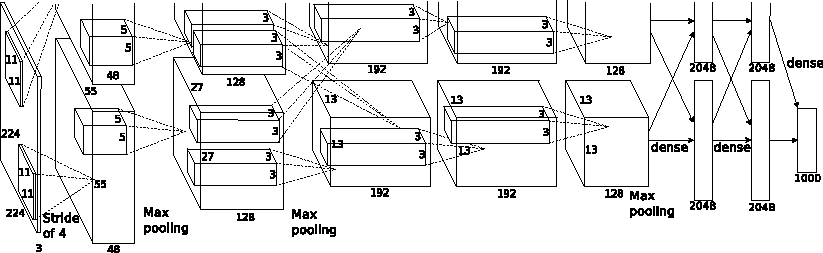
\includegraphics[width=\textwidth]{figures/networks/alexnetarchitecture}
  \caption{ AlexNet 卷积神经网络模型\cite{krizhevsky2012imagenet}}
  \label{fig:cnn_network}
\end{figure}

% 它同时,它可以通过池化(合并相邻特征)减少计算复杂度。
% 深度卷积神经网络与的两个主要区别是其

% ,这部分为需要进行主要设计,也是各种神经网络模型的主要区别之处。
% 为了增强其泛化能力,一般情况下有扩增路径(将多个分支包含在架构中)、金字塔形状(在整个架构中应该有一次整体的平滑的下采样,而且该下采样应该与信道数量的增长结合起来)、规范层输入(使层输入标准化,使所有输入样本更加平等)等各种设计法则,此部分需要根据实际问题以及测试结果不断调整。

\subsection{卷积}

深度卷积神经网络在特征提取过程中一个主要操作为卷积,在前向计算过程中,对于输入的一定区域的隐藏层的特征向量$x$和滤波器(权重)$w$ 点乘后得到新的特征向量,然后滑过一个个滤波器,以产生输出特征向量。
权重实际上是一个四维张量,第一维$ F $是卷积输入层的特征向量的数量,另一维$ F_p $是卷积输出层的特征向量的数量,另外两维是在宽度和高度方向给出的卷积核的大小,也称作感受野。

对于传统的神经网络,每个输入元素会连接到每个隐藏神经元。然而,在卷积神经网络中,我们只是把输入数据进行小的、局部区域的连接,也即第一个隐藏层中的每个神经元会连接到一个输入神经元的一个区域。这个输入向量的区域被称为隐藏神经元的局部感受野。它是输入向量上的一个小窗口,对于每个连接学习一个权重而隐藏神经元同时也学习一个总的偏置。通过在整个输入频谱数据上交叉移动局部感受野,可以构建起第一个隐藏层。

感受野允许用一个子集来代替整个输入数据。它的目的是在输入数据中搜索相似的模式,而不管模式在哪里,也即平移不变性。输出图像的宽度和高度也由步长(stride)确定,步长为在进行再次应用卷积运算之前在垂直、水平方向上滑动的像素的数目。我们以图\ref{fig:conv}这个对一个图像进行二维卷积的操作来介绍卷积运算。

% TODO: \textcolor{red}{统一公式变量等}

\begin{figure}[!t]
	\centering
  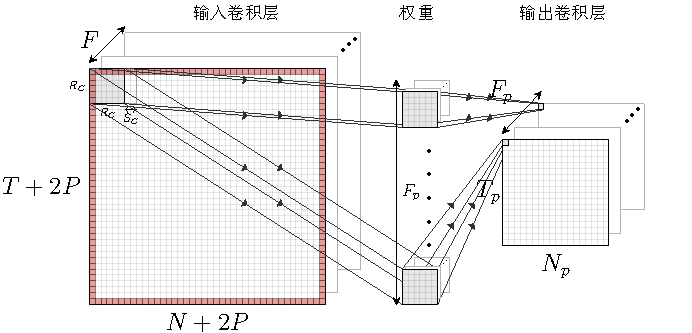
\includegraphics[width=\textwidth]{figures/networks/conv}
	\caption{卷积示意图}
	\label{fig:conv}
\end{figure}

其中 $R_C$ 为卷积感受野的大小,$S_C$为卷积的步长。
根据输入高度$ T $和宽度$ N $,可以计算输出图像的高度和宽度:
\begin{align}
  N_p&=\frac{N+2P-R_C}{S_C}+1 \;,&
  %
  T_p&=\frac{T+2P-R_C}{S_C}+1\;
\end{align}

通常对输入数据进行边界扩充(padding)来使得输入特征图的宽度和高度满足$ N = N_p = T = T_p $,这样当前进步长$ S_C = 1 $时,可以得到
\begin{align}
P&=\frac{R_C-1}{2}\;
\end{align}
对于一个给定的层$ L_n $,卷积运算的计算过程如下:
\begin{align}
y_{f\,l\,m}^{(\nu)}&=\sum^{F_\nu-1}_{f'=0}\sum^{R_C-1}_{j=0}\sum^{R_C-1}_{k=0}
%
w^{(o)f}_{f'\,j\,k}h^{(\nu)}_{f'\,S_Cl+j\,S_Cm+k}\;
\end{align}
其中$ o $表示网络中的第$ o + 1 $个卷积核。
$\nu \in [0,N-1 ]$ 表示网络中的第 $\nu$个隐层,$f\in[0,F_{\nu+1}-1]$为输入卷积层的第$f$个特征图, $l\in[0,N_{\nu+1}-1 ]$为输入卷积层的第$v$个特征图的宽度单位, $m\in[0,T_{\nu+1}-1 ]$为输入卷积层的第$v$个特征图的高度单位。 因此可以得到 $S_Cl+j\in[0,N_\nu-1 ]$, $S_Cl+m\in[0,T_\nu-1 ]$。于是可以通过添加激活函数计算隐藏单元的输出。
考虑到边界填充可以得到下式
\begin{align}
h_{f\,l+P\,m+P}^{(\nu+1)}&=f\left(y_{f\,l\,m}^{(\nu)}\right)\;
\end{align}
每个滤波器只关心数据的部分特征,当出现它学习到的特征的时候,就会呈现激活态。

\subsection{共享权重和偏置}
上面已经说过对于每个隐藏神经元具有一个偏置和连接到它的局部感受野的权重,同时对于该层的所有的隐藏神经元中每一个使用相同的权重和偏置。也即对第$j$个隐藏神经元,输出为:
\begin{equation}
  h_j = f(b+\sum_{m=1}^M w_m y_{j+m})
\end{equation}
这里$f$是神经元的激活函数,$b$是偏置的共享值,$w_m$是一个共享权重的$1\times M$向量,$y_k$表示位置$k$的输入激活值。
\textcolor{red}{这意味着第一个隐藏层的所有神经元检测完全相同的特征,只是在输入数据的不同位置,因此卷积网络可以很好地适应数据偏移情况。}

\subsection{池化}
我们在通过卷积获得了特征之后,下一步我们希望利用这些特征去做分类。理论上讲,人们可以用所有提取得到的特征去训练分类器,例如Softmax分类器(多分类的逻辑回归分类器),但这样做面临着计算量的挑战,除此以外过多的特征向量,也容易导致过拟合。
由于本文的雷达信号具有一种“静态性”属性,在一个数据区域有用的特征极有可能在另一个区域同样适用。因此,为了描述数据量较多的数据,一个很自然的想法就是对不同位置的特征进行聚合统计,例如,可以计算频谱数据上一段频率范围内的某个特征的最大值(或平均值)。这些经过采样的统计特征相比使用所有提取得到的特征不仅具有低得多的维度,同时还不容易过拟合,在一定程度上会改善结果。这种聚合的操作称为池化。
池化操作是卷积神经网络中一种常用的用来对数据进行降维处理的方法。一般有平均池化和最大池化,主要过程为选取输入特征向量的$F$一个池化感受野$R_P$和步长$S_P$选取其最大或者平均元素来代表该区域,得到输出特征向量$F_p=F$,其中宽度 $N_p<N$,高度 $T_p<T$。在池化操作过程中,我们一般不考虑输入隐藏层的边界扩充值,因此在公式\ref{equ:pool}中存在 $+P$ 这一部分。

对于给定的第$\nu$个平均池化操作的公式如下:
\begin{align}
y_{f\,l\,m}^{(\nu)}&=\sum^{R_P-1}_{j,k=0} h_{f\,S_P l+j+P\,S_Pm+k+P}^{(\nu)}\;
\label{equ:pool}
\end{align}
最大池化的公式为:
\begin{align}
y_{f\,l\,m}^{(\nu)}&=\max^{R_P-1}_{j,k=0} h_{f\,S_P l+j+P\,S_Pm+k+P}^{(\nu)}\;
\label{equ:maxpool}
\end{align}
其中,$\nu \in [0,N-1 ]$ 表示网络中的第 $\nu$个隐层,$f\in[0,F_{\nu+1}-1]$, $l\in[0,N_{\nu+1}-1 ]$ 以及 $m\in[0,T_{\nu+1}-1 ]$。因此有 $S_Pl+j\in[0,N_\nu-1 ]$, $S_Pl+m\in[0,T_\nu-1 ]$。
最大池化是最常用的一种池化方式,本文所用的神经网络结构均使用最大池化。
对于第$t$次批采样,我们用$j^{(t)(p)}_{_{flm}},\,k^{(t)(p)}_{_{flm}}$来表示在 $l,m$处特征向量图的最大值,则公式\ref{equ:maxpool}变为下式:
\begin{align}
h_{f\,l+P\,m+P}^{(t)(\nu+1)}&=y_{f\,l\,m}^{(t)(\nu)}=
%
h^{(t)(\nu)}_{f\,S_P l+j^{(t)(p)}_{_{flm}}+P\,S_Pm+k^{(t)(p)}_{_{flm}}+P}\;
\end{align}

\begin{figure}[!t]
	\centering
	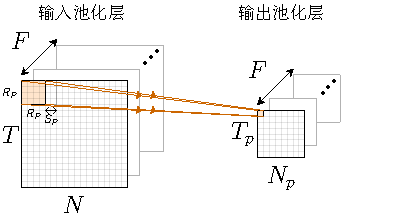
\includegraphics[width=\textwidth]{figures/networks/pool}
	\caption{池化示意图}
	\label{fig:pool}
\end{figure}

深度卷积神经结构具有过拟合的自然趋势,虽然可以通过权重共享来减少参数的数量。但是由于大多数情况下,估计集的数量比训练集大一个数量级,使得神经网络模型的泛化能力不足。在每个训练迭代中,每个隐藏单元以预定概率被随机删除,删除后学习过程继续。这些被称作dropout的随机扰动有效地防止了神经网络学习过程的依赖关系,并在隐藏的单元之间创建了复杂的关系。这样增加了网络模型的复杂度,从而提高深度神经网络模型的泛化能力。


\subsection{激活函数}

在公式\ref{equ:fp2}中,$f(x)$被用于每一个神经元节点,因此激活函数的选择是构建卷积神经网络模型的一个非常重要的方面。我们在本节介绍几种常用的激活函数。

\subsubsection{sigmoid 激活函数}

在传统人工神经网络中常用的激活函数为sigmoid激活函数(S型激活函数),其取值范围为$(0,1)$,其定义如下式:

\begin{align}
f(x)&=\sigma(x)=\frac{1}{1+e^{-x}}\;
\end{align}
对其求导可以得到:
\begin{align}
\sigma'(x)&=\sigma(x)\left(1-\sigma(x)\right)\;
\end{align}

\begin{figure}[hbt]
	\centering
	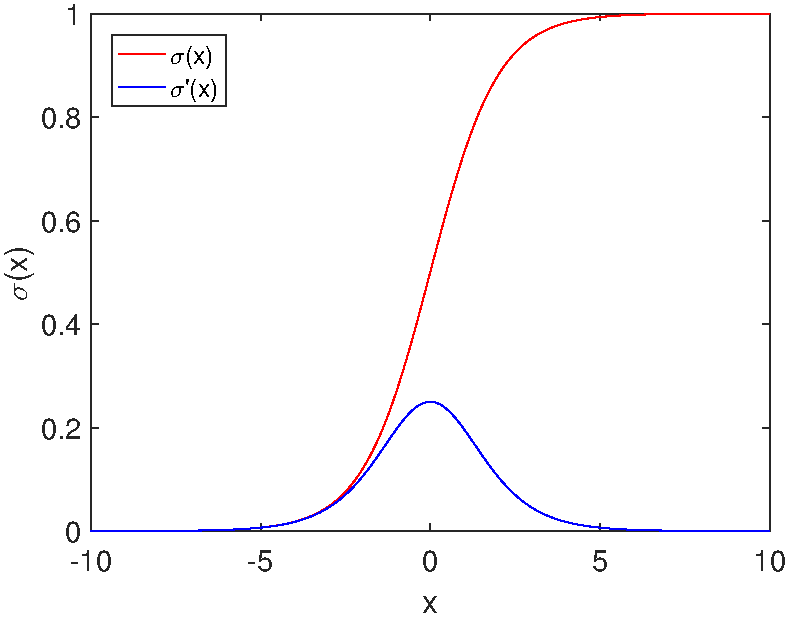
\includegraphics[width=0.4\textwidth]{figures/networks/sigmoid}
	\caption{sigmoid 激活函数及其导数}
	\label{fig:sigmoid}
\end{figure}

\subsubsection{ tanh 激活函数}

tanh 激活函数的取值范围为 $(-1,1)$,其定义如下:
\begin{align}
f(x)&=\tanh(x)=\frac{1-e^{-2x}}{1+e^{-2x}}\;
\end{align}
对其求导可以得到:
\begin{align}
\tanh'(x)&=1-\tanh^2(x)\;
\end{align}

\begin{figure}[!t]
	\centering
	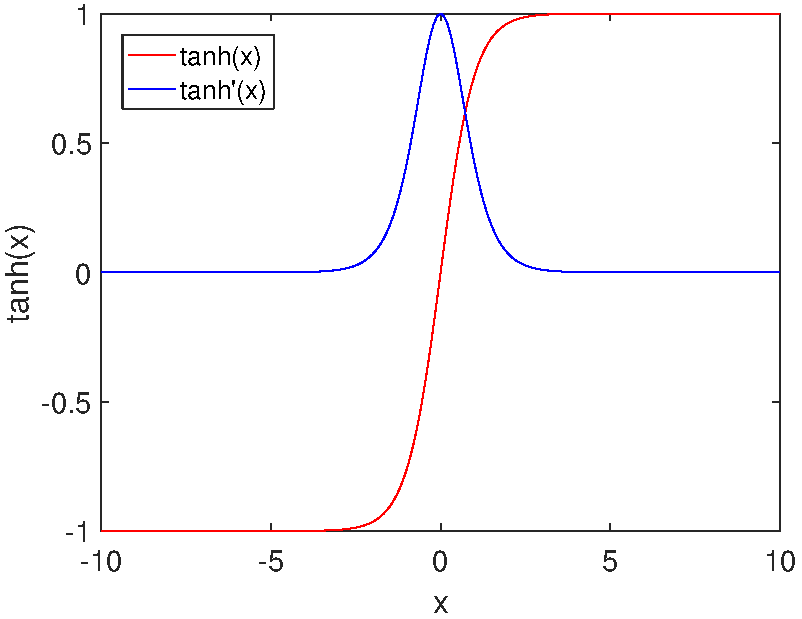
\includegraphics[width=0.4\textwidth]{figures/networks/tanh2}
	\caption{tanh2 激活函数及其导数}
	\label{fig:tanh2}
\end{figure}

\subsubsection{ReLU 激活函数}

ReLU(Rectified Linear Unit)的取值范围为$[0,+\infty)$,其定义如下式:
\begin{align}
f(x)&={\rm ReLU}(x)=\begin{cases}
      x & x\geq 0 \\
      0& x<0
   \end{cases}\;
\end{align}
对其求导可以得到:
\begin{align}
{\rm ReLU}'(x)&=\begin{cases}
      1 & x\geq 0 \\
      0 & x<0
   \end{cases}\;
\end{align}

\begin{figure}[!t]
	\centering
	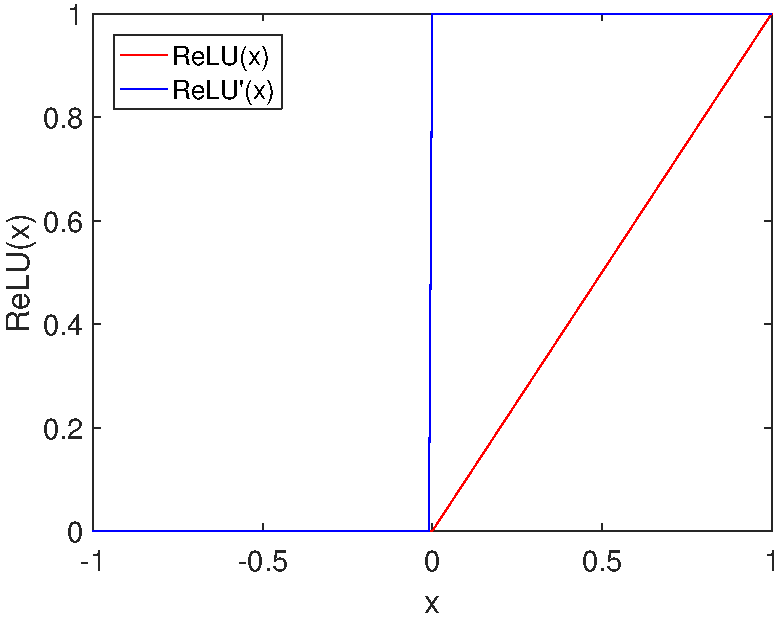
\includegraphics[width=0.4\textwidth]{figures/networks/ReLU}
	\caption{ReLU 激活函数及其导数}
	\label{fig:ReLU}
\end{figure}

ReLU具有优于传统激活函数的几个优点:更快的计算速度和更有效的梯度传播(它们不像S形单元那样饱和),生物学可能性和稀疏激活结构。尽管它结构简单,但仍然保持足够的辨别性质。其缺点之一是随机权重的初始状态,多个单位可能过早地落入死区(零输出的恒定梯度)。因此,当与整个连接层进行全连接时,Sigmod激活函数的效果更好。

\subsection{网络的训练与学习}
% \textcolor{red}{添加文字描述,关于梯度下降算法。}
参照上文的符号定义,用符号$x $表示训练输入的向量集,$w$表示所有的网络中权重的集合,$b$ 是所有的偏置,用$y=f(w\cdot x + b)$ 表示对应的期望输出。学习算法的主要目的是找到一个权重$w$和偏置$b$使得网络的输出$y$ 可以拟合所有的训练输入$x$。为此可以定义一个损失函数或代价函数(loss function)$C(w,b)$。针对于不同的问题可以选取不同的损失函数,公式\ref{equ:loss_mse}利用均方误差函数作为损失函数。
\begin{equation}
C(w,b)\equiv \frac{1}{2n}\sum_x||y-a||^2
\label{equ:loss_mse}
\end{equation}
其中, $n$是训练输入数据的个数,$a$表示当输入为$x$时的输出向量。

从定义可以看出,$C(w,b) $越小说明分类越准确,那么训练神经网络的目的就是找到使得损失函数 $C(w,b)$最小的权重和偏置。
为了求解该问题,将上述问题一般化,原问题变为最小化任意的具有 $m $个变量的多元实值函数 $C(v) $, $v=v_1,v_2,\dots,v_m $。这种具有大量变量的函数的解析解的求解是极其复杂的,一个比较合理的思路为利用数值计算的方法求取其极值点。每次对于$C $中的自变量 添加一个微小的变化$\Delta v $,根据此变化反映出来的$C $的变化$\Delta C $更新下次的微小变化,从而使得$C $ 可以持续减小。对$C $中自变量的变化$\Delta v=(\Delta v_1,\dots,\Delta v_m)^T $ , $\Delta C $将会变为
\begin{equation}
    \Delta C \approx \nabla C \cdot \Delta v
    \label{equ:gradient1}
\end{equation}
,这里的梯度$\nabla C $ 定义如下:
\begin{equation}
\nabla C \equiv (\frac{\partial C}{\partial v_1},\dots,\frac{\partial C}{\partial v_m})^T
\end{equation}
其把$v$的变化关联为$C$的变化,假设选取$\Delta v=-\eta \nabla C $,其中的$\eta $是学习率,一般取一个很小的正数,则公式\ref{equ:gradient1}变为:
\begin{equation}
\Delta C \approx -\eta\nabla C\cdot\nabla C=-\eta||\nabla C||^2 \leq 0
\end{equation}
也即如果利用更新规则$v \rightarrow v'=v-\eta \nabla C$,$C$会持续减小,此更新规则即为最基本的学习算法,梯度下降算法。
图\ref{fig:gradient-descent}展示了梯度下降的示意图,其跟随当前位置最陡的下降的方向也即负梯度,其中学习率$ \eta $描述在每个迭代步骤中下降的步长。
可以根据选择不同的损失函数 $C $或者通过计算来完成学习率的选择等各种技术对学习算法进行优化。
\begin{figure}[hbt]
	\centering
  \includestandalone[width=0.7\textwidth]{figures/networks/gradient-descent}
  \caption{梯度下降示意图}
    \label{fig:gradient-descent}
\end{figure}

根据梯度下降的思想,我们可以结合卷积神经网络中的反向传播,获得对于神经卷积神经网路的训练流程图,如图\ref{fig:cnn_train}所示。
\begin{figure}[hbt]
	\centering
	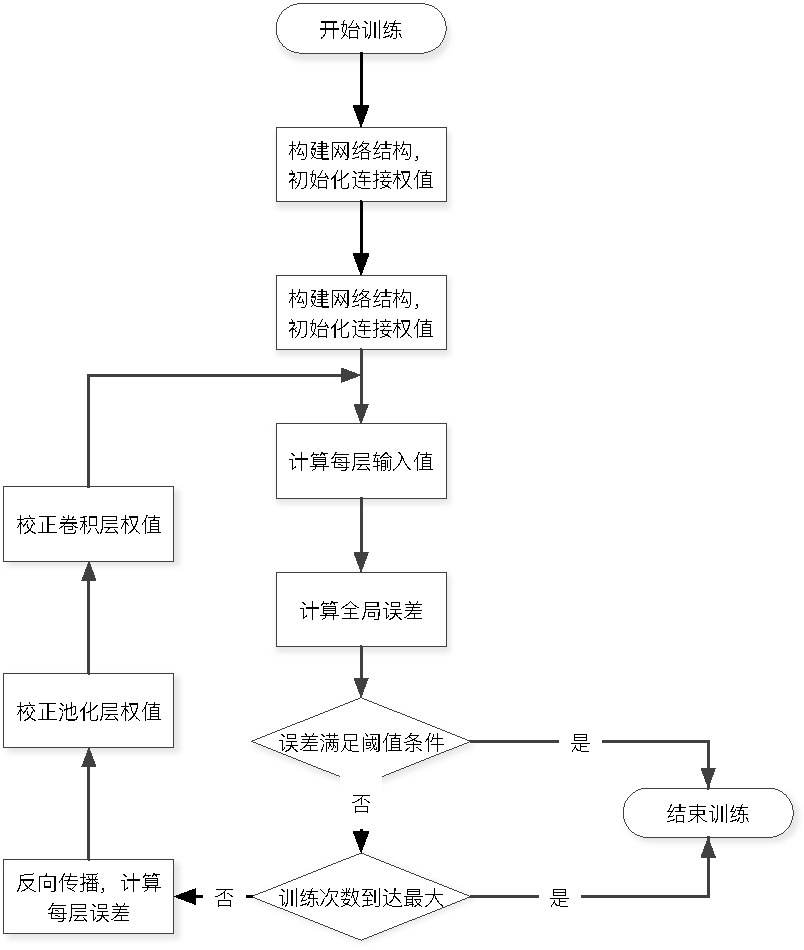
\includegraphics[width=\textwidth]{figures/networks/cnn_train}
	\caption{深度卷积神经网络算法训练流程图-----------该图需要修改}
	\label{fig:cnn_train}
\end{figure}
\section{小结}
本章介绍了深度学习的相关基础。首先是其基本分类,然后针对于本文利用的深度卷积神经网络,介绍了传统的神经元的结构和卷积神经网络基于此的改进。在最后讨论了深度卷积神经网络在雷达信号处理中的应用。
